%!TEX encoding = UTF-8 Unicode

\documentclass[journal]{IEEEtran}

\usepackage[T1]{fontenc} % output - specifies encoding used in fonts; needs full LaTeX distribution to produce good-looking output
\usepackage[utf8]{inputenc} % input - type accented characters directly from keyboard
\usepackage[english]{babel} % internationalization - hyphenation, typographic rules for one or more languages

\usepackage[nounderscore]{syntax} % definition of the context-free grammar

\usepackage[
    backend=biber, % bibliography engine
    style=ieee, % bibliography style .bbx and citation style .cbx
    hyperref, % make citations and references clickable - requires hyperref pkg
    maxbibnames=99, % 99 = display all authors of multi-author articles
    doi=false, % do not display DOI
    isbn=false, % do not display ISBN
    ]
        {biblatex} % note: incompatible with ucs (-> utf8x), natbib
\usepackage[
    autostyle] % adapt citation style to current document language
        {csquotes} % Context Sensitive Quotations; provides biblatex \enquote{}

\usepackage[nolist]{acronym}
\usepackage{amsmath}
\usepackage{amssymb}
\usepackage{bm} % bold math
\usepackage{booktabs}
\usepackage{graphicx}
\usepackage{hyperref}
\usepackage{siunitx}
\usepackage{subfig}
\usepackage{tabularx}
\usepackage{url}

\usepackage{tikz}
\usetikzlibrary{matrix,positioning}
\usetikzlibrary{decorations.text}
\usetikzlibrary{shapes.geometric}
\usetikzlibrary{fit}
\tikzstyle{circle}=[shape=circle,minimum size=0.7cm,very thick]
\tikzstyle{every path}=[very thick]
\usetikzlibrary{arrows}

\usepackage{hyperref}
\usepackage[update,prepend]{epstopdf}
\graphicspath{{figures/}}

\addbibresource{lang_journal_bibliography.bib}

% custom commands and frequent expressions that require typesetting care
\newcommand{\actioneffect}{action--effect}
\newcommand{\AffWords}{Affordance--Words}
%\newcommand{\affwords}{affordance--words}
\newcommand{\FB}{Forward--Backward}
\newcommand{\HR}{Human--Robot}
\newcommand{\HRI}{\HR{} Interaction}
\newcommand{\hh}{human--human}
\newcommand{\hr}{human--robot}
\newcommand{\hri}{\hr{} interaction}
\newcommand{\ObjAct}{Object--Action}
\newcommand{\objecthand}{object--hand}
\newcommand{\SensMot}{Sensory--Motor}

\newcommand{\phmm}{\ensuremath{P_{\text{HMM}}}}
\newcommand{\pbn}{\ensuremath{P_{\text{BN}}}}
\newcommand{\pcomb}{\ensuremath{P_\text{comb}}}
\newcommand{\xinf}{\ensuremath{X_\text{inf}}}
\newcommand{\xobs}{\ensuremath{X_\text{obs}}}
\newcommand{\xlat}{\ensuremath{X_\text{lat}}}

%\newcommand{\given}{\ensuremath{|}} % Giampiero, without space around bar
\newcommand{\given}{\ensuremath{\mid}} % Giovanni, with space around bar

% list of acronyms
\begin{acronym}
\acro{AI}{Artificial Intelligence}
\acro{BN}{Bayesian Network}
\acro{CFG}{context-free grammar}
\acro{HMM}{Hidden Markov Model}
\acro{MTRNN}{Multiple Timescales Recurrent Neural Network}
\acro{OAC}{\ObjAct{} Complex}
\acrodefplural{OAC}{\ObjAct{} Complexes}
\acro{PDF}{Probability Density Function}
\end{acronym}

%%%%%%%%%%%%%%%%%%%%%%%%%%%%%%%%%%%%%%%%%%%%%%%%%%%%%%%%%%%%%%%%%%%%%%%%%%%%%%%%
\begin{document}

\title{Beyond the Self: Using Grounded Affordance Knowledge to Interpret Others' Actions}

\author{Giovanni~Saponaro,~\IEEEmembership{Student Member,~IEEE,}
        Lorenzo~Jamone,~\IEEEmembership{Member,~IEEE,}
        Alexandre~Bernardino,~\IEEEmembership{Member,~IEEE}
        Giampiero~Salvi,~\IEEEmembership{Member,~IEEE}
\thanks{G.~Saponaro, and A.~Bernardino are with the
Institute for Systems and Robotics, Instituto Superior Técnico,
Universidade de Lisboa, Lisbon, Portugal, e-mail: \{gsaponaro,alex\}@isr.tecnico.ulisboa.pt.

L.~Jamone is with ARQ~(Advanced Robotics at Queen Mary), School of Electronic Engineering and Computer Science, Queen Mary University of London, United Kingdom
and with the
Institute for Systems and Robotics, Instituto Superior Técnico, Universidade de Lisboa, Lisbon, Portugal,
e-mail: l.jamone@qmul.ac.uk.

G.~Salvi is with the Speech, Music and Hearing Department,
KTH Royal Institute of Technology, Stockholm, Sweden,
e-mail: giampi@kth.se.
}}

% make the title area
\maketitle

%%%%%%%%%%%%%%%%%%%%%%%%%%%%%%%%%%%%%%%%%%%%%%%%%%%%%%%%%%%%%%%%%%%%%%%%%%%%%%%%
\begin{abstract}
With time and with social experience, children develop narrative abilities~(e.g., describing a physical event, using adequate grammar to that effect, producing the correct utterances).
On the other hand, social robots still have a way to go in that regard, because of the difficulty of modeling and interpreting the real world, which is characterized by being highly variable, unstructured, and unpredictable.
%Cognitive robots operating in unstructured environments

We hypothesize that a humanoid robot can generalize its previously-acquired knowledge of the world~(objects, actions, effects, verbal descriptions) to the cases when it observes a human agent performing familiar actions in a shared \hr{} environment.

We propose a probabilistic method to fuse self-learned knowledge with the observation of other human agents.
We report results about how our model is able to learn and do inference from these conjoint sources of information, as well as generating verbal descriptions of \hr{} collaboration scenarios with manipulative actions.
\end{abstract}

\begin{IEEEkeywords}
affordances, gestures, humanoid robots, language learning.
\end{IEEEkeywords}

%%%%%%%%%%%%%%%%%%%%%%%%%%%%%%%%%%%%%%%%%%%%%%%%%%%%%%%%%%%%%%%%%%%%%%%%%%%%%%%%
%!TEX encoding = UTF-8 Unicode

\section{Introduction}
\label{sec:intro}

TODO shorten

% paragraph about HRC, understanding others, communication for cooperation
\IEEEPARstart{C}{ooperation}, the ability of working successfully in groups, is a tenet of human society~\cite{turner:1975}.
This skill is acquired around the second year of life, when children develop an ability to coordinate themselves with peers or adult caregivers in shared problem-solving activities and social games, not only by mere behavioral coordination, but also by
%showing knowledge about how the different roles are interrelated, as well as
employing communicative strategies~\cite{melis:2010:rstb}.
In adulthood, understanding one another is a fundamental pre-requisite for success.
Team members typically agree on common goals~(e.g., through verbal and non-verbal communication), they work towards the execution of these goals in a coordinated way, and they understand each other's physical actions~(e.g., body movements) towards the realization of the final target.
Human team coordination and mutual understanding is effective~\cite{ramnani:2004:natureneuro} because of~(i) the capacity to adapt to unforeseen events in the environment, and reactively re-plan one's actions, and~(ii) a common motor repertoire and action model, which permits us to understand a partner's physical actions and manifested intentions as if they were our own.
% GLU
%Robotics is progressing fast, with a steady and systematic shift from the industrial domain to domestic, public and leisure environments~\cite[ch.~65, Domestic Robotics]{siciliano:2016:handbook2}. Application areas that are particularly relevant and being researched by the scientific community include: robots for people's health and active aging, mobility, advanced manufacturing~(Industry~4.0). In short, all domains that require direct and effective \hri{} and communication (including language and gestures~\cite{matuszek:2014:aaai}).
%However, robots have not reached the level of performance that would enable them to work with humans in routine activities in a flexible and adaptive way, for example in the presence of sensor noise, or unexpected events not previously seen during the training or learning phase. One of the reasons to explain this performance gap between \hh{} teamwork and a \hr{} teamwork is in the collaboration aspect, i.e., whether the members of a team understand one another. Humans have the ability of working successfully in groups. They can agree on common goals~(e.g., through verbal and non-verbal communication), work towards the execution of these goals in a coordinated way, and understand each other's physical actions~(e.g., body gestures) towards the realization of the final target. Human team coordination and mutual understanding is effective~\cite{ramnani:2004:natureneuro} because of~(i) the capacity to \emph{adapt} to unforeseen events in the environment, and re-plan one's actions in real time if necessary, and~(ii) a common motor repertoire and action model, which permits us to understand a partner's physical actions and manifested intentions as if they were our own~\cite{saponaro:2013:crhri}.

% paragraph about social sobots, need for learning/adaptation of language
Even though social robots\footnote{A social robots is ``[a robot that is] able to communicate and interact with us, understand and even relate to us, in a personal way. [It] should be able to understand us and itself in social terms''~\cite{breazeal:2002:dsr}.} are becoming more present in domestic and public environments~(thanks to the rapid technical advancements that touch all aspects of robotics: sensors, actuators, and algorithms), the performance of \hh{} teams is still superior to that of \hr{} teams.
Putting socially intelligent machines alongside common human users~(as opposed to specialized factory technicians as has been done in industry since the 1960s), bears challenges.
For instance, the communication skills possessed by a robot cannot be entirely pre-programmed, because we cannot possibly model all the imaginable verbal and non-verbal~(e.g., gestures) cues that can take place during \hri, due to the richness of language and the high variability of the real world outside of structure research laboratories and factories.
For this reason, it is necessary to have robots that \emph{learn} elements and properties of language and communication, and the ability to link these verbal elements with other skills, such as other perceptual modalities~(e.g., vision of objects of the world, vision of other agents' physical actions) and manipulation abilities~(e.g., grasping objects and moving them in order to achieve a goal)~\cite{steels:2003:trendscogsci}.

% paragraph about developmental robotics
One way to endow robots with adaptability and learning in the real world is the growing field of developmental robotics~\cite{lungarella:2003:devrobsurvey,cangelosi:2015:devrobbook}.
It takes inspiration from the progressive learning phenomena observed in children's mental development~(e.g., the understanding of language, the acquisition of manipulation skills, the understanding of others' actions), and investigates how to model the evolution and acquisition of these increasingly complex cognitive processes.
In this line of research, which we follow, robots are experimental platforms.
They are used to verify theoretical models of emergence and development of cognition.
The rationale is the following: if a model is instantiated inside a system physically embedded in the real world, many things can be learned about its strengths and limitations.
This is often accompanied by probabilistic and statistical methods~\cite{pearl:2014:probabilistic}.

% paragraph about neuroscience, and correspondence problem in robotics
In neuroscience research, visuomotor neurons~(i.e., neurons that are activated by visual stimuli) have been a subject of ample study~\cite{rizzolatti:2001:nrn}.
Mirror neurons are one class of such neurons that responds to action and object interaction, both when the agent acts and when it observes the same action performed by others, hence the name ``mirror''.
We show that, using this theory, a robot can first acquire knowledge by sensing and self-exploring its surrounding environment~(e.g., by interacting with available objects and building up an affordance representation of the interactions and their outcomes) and, as a result, the robot is capable of generalizing its acquired knowledge while observing another agent~(e.g., a human person) who performs similar physical actions to the ones executed during prior robot training.
This tackles the so-called correspondence problem~\cite{nehaniv:2002:correspondence} in our simple collaboration scenario, assuming that the two agents have a similar body~(i.e., a humanoid robot and a human) and operate on a shared space~(i.e., a table accessible by both agents' arms).

% paragraph summarizing our contributions and comparing with the GLU article
This article is an extention of our recent work~\cite{saponaro:2017:glu}.
We combine robot ego-centric learning about language and object affordances~\cite{salvi:2012:smcb} with the observation of external agents by gesture recognition~\cite{saponaro:2013:crhri}.
Our novel contributions are:
(i)~a probabilistic method to fuse self-learned knowledge of language and object affordances, with socially aware information of others' physical actions~(in the form of uncertain soft evidence);
(ii)~experimental findings showing the reasoning power of our combined system, which is able to make inferences and predictions over affordances and words% by incorporating the estimation of external agents
; and
(iii)~the possibility of generating verbal descriptions from the estimated word probabilities, with emergence of non-trivial language properties such as congruent/incongruent conjunctions, synonyms between two consecutive sentences speaking about the same concepts.

Furthermore, we make our human action data and probabilistic reasoning code publicly available\footnote{\url{https://github.com/gsaponaro/tcds-gestures} - this page access will be made available at publication time.} in the interest of reproducibility.

The article is structured as follows. TODO ToC

%GLU
% This work takes inspiration from the theory of mirror neurons, and contributes towards using it on humanoid and cognitive robots. We show that a robot can first acquire knowledge by sensing and self-exploring its surrounding environment~(e.g., by interacting with available objects and building up an affordance representation of the interactions and their outcomes) and, as a result, the robot is capable of generalizing its acquired knowledge while observing another agent~(e.g., a human person) who performs similar physical actions to the ones executed during prior robot training. Fig.~\ref{fig:experimental_setup} shows the experimental setup.

%PHOTOS FROM OCTOBER 2017, NOT USED
% Below are the human-robot images from the external view (camera on a tripod)
% TODO: if we don't use them, purge seq2-*.png from the repo history
% \begin{figure*}
%     \centering
%     \subfloat
%     { \includegraphics[width=\myWidth\linewidth]{seq2-grasp-11} } \quad
%     %
%     \subfloat
%     { \includegraphics[width=\myWidth\linewidth]{seq2-grasp-12} } \quad
%     %
%     \subfloat
%     { \includegraphics[width=\myWidth\linewidth]{seq2-grasp-13} } \\
%     %
%     \subfloat
%     { \includegraphics[width=\myWidth\linewidth]{seq2-grasp-14} } \quad
%     %
%     \subfloat
%     { \includegraphics[width=\myWidth\linewidth]{seq2-grasp-15} } \quad
%     %
%     \subfloat
%     { \includegraphics[width=\myWidth\linewidth]{seq2-grasp-16} }
%     \caption{grasp}
% \end{figure*}
%
% \begin{figure*}
%     \centering
%     \subfloat
%     { \includegraphics[width=\myWidth\linewidth]{seq2-tap-22} } \quad
%     %
%     \subfloat
%     { \includegraphics[width=\myWidth\linewidth]{seq2-tap-23} } \quad
%     %
%     \subfloat
%     { \includegraphics[width=\myWidth\linewidth]{seq2-tap-24} } \\
%     %
%     \subfloat
%     { \includegraphics[width=\myWidth\linewidth]{seq2-tap-25} } \quad
%     %
%     \subfloat
%     { \includegraphics[width=\myWidth\linewidth]{seq2-tap-26} } \quad
%     %
%     \subfloat
%     { \includegraphics[width=\myWidth\linewidth]{seq2-tap-27} }
%     \caption{tap}
% \end{figure*}
%
% \begin{figure*}
%     \centering
%     \subfloat
%     { \includegraphics[width=\myWidthTwo\linewidth]{seq2-touch-2} } \quad
%     %
%     \subfloat
%     { \includegraphics[width=\myWidthTwo\linewidth]{seq2-touch-3} } \quad
%     %
%     \subfloat
%     { \includegraphics[width=\myWidthTwo\linewidth]{seq2-touch-4} } \quad
%     %
%     \subfloat
%     { \includegraphics[width=\myWidthTwo\linewidth]{seq2-touch-5} } \\
%     %
%     \subfloat
%     { \includegraphics[width=\myWidthTwo\linewidth]{seq2-touch-6} } \quad
%     %
%     \subfloat
%     { \includegraphics[width=\myWidthTwo\linewidth]{seq2-touch-7} } \quad
%     %
%     \subfloat
%     { \includegraphics[width=\myWidthTwo\linewidth]{seq2-touch-8} } \quad
%     %
%     \subfloat
%     { \includegraphics[width=\myWidthTwo\linewidth]{seq2-touch-9} }
%     \caption{touch}
% \end{figure*}


%%%%%%%%%%%%%%%%%%%%%%%%%%%%%%%%%%%%%%%%%%%%%%%%%%%%%%%%%%%%%%%%%%%%%%%%%%%%%%%%
%!TEX encoding = UTF-8 Unicode

\section{Related Work}
\label{sec:related_work}

% collaboration and language
Human cooperation is a phenomenon that we often take for granted~(at least in adults), possibly because it is widespread and intimately embedded into human societies.
However, this non-trivial skill is greatly facilitated, and influenced, by human language~\cite{mueller:2000:psych}.
For instance, educational research has shown that, when language is used as a cultural tool for intellectual tasks in preteen students, discursive interaction enables collective thinking to become more effective, also fostering individual reasoning and faster learning~\cite{rojas:2003:ijer}. % related: leman:2000 (age 7--9)
%~(i.e., a highly elaborated, complex yet efficient communication system)

% mirror neurons, link to robotics, correspondence problems
The ability to understand and interpret our peers has also been studied in neuroscience and psychology, focusing on visuomotor neurons~\cite{rizzolatti:2001:nrn}, i.e., neurons that are activated by visual stimuli.
Mirror neurons respond to action and object interaction, both when the agent acts and when it observes the same action performed by others, hence the name ``mirror''.
They are based on the principle that perceptual input can be linked with the human action system for predicting future outcomes of actions, i.e., the effect of actions, particularly when the person possesses concrete prior personal experience of the actions being observed in others~\cite{aglioti:2008:basketball,knoblich:2001:psychsci}.
Applying the mirror neuron theory in robotics, as we and others do~\cite{gazzola:2007:neuroimage,lopes:2009:ab}, an agent can first acquire knowledge by sensing and self-exploring its surrounding environment, %~(e.g., by interacting with available objects and building up an affordance representation of the interactions and their outcomes)
afterwards it can employ that learned knowledge to novel observations of another agent~(e.g., a human person) who performs similar physical actions to the ones executed during prior training.
This tackles the so-called correspondence problem~\cite{nehaniv:2002:correspondence}, in our case in a simple collaboration scenario, assuming that the two agents have a similar body~(i.e., a humanoid robot and a human) and operate on a shared space~(i.e., a table accessible by both agents' arms).
Some authors have studied this concept under the deep learning paradigm.
In~\cite{kim:2017:nn}, a \ac{MTRNN} is proposed to have an artificial simulated agent infer human intention from joint information about object, their potential opportunities~(i.e., their affordances) and human actions.
However, in that work a virtual simulation able to produce large quantities of data was used, but a simulator, by nature, cannot model all the physical events and unpredictability of the real world.
In contrast, we use real, noisy data acquired from robots and sensors to validate our model~(we also make the data and implementation publicly available).
Recently, DeepMind and Google published a method~\cite{santoro:2017:relational_reasoning} to perform relational reasoning on images, i.e., a system that learns to reason about entities and their mutual relations, with the ability of providing answers to questions such as ``Are there any rubber things that have the same size as the yellow metallic cylinder?''.
That work is very powerful from the point of view of cognitive systems, vision and language.
Our approach is different because (i)~we focus on \emph{robotic} cognitive systems, including manipulation and the uncertainties inherent to robot vision and control, and (ii)~we follow the developmental paradigm and the embodiment hypothesis~\cite{lungarella:2003:devrobsurvey}, meaning that, leveraging the fact that a human and a humanoid share similar body structures, we relate words with the robot's \emph{sensorimotor} experience, rather than sensory only~(purely images-to-text).

% robot affordances
In robotics and cognitive systems research, both object-directed action recognition in external agents~\cite{koppula:2013:ijrr} and the incorporation of language in \hr{} systems~\cite{harnad:1990,matuszek:2014:aaai} have received ample attention.
A growing interest is devoted to robots that learn new cognitive skills and improve their capabilities by interacting autonomously with the surrounding environment.
Robots operating in the unstructured world may understand available opportunities conditioned on their body, perception and sensorimotor experiences: the intersection of these elements gives rise to object \emph{affordances}~(action possibilities), as they are called in psychology~\cite{gibson:2014}.
The advantage of robot affordances lies in the ability to capture essential functional properties of environment objects in terms of the actions that the agent is able to perform with them, allowing to generalize knowledge to never-before-seen scenarios, thus exhibiting learning~\cite{montesano:2008,jamone:2016:tcds}.
%Some authors have suggested a computational model called \acp{OAC}~\cite{kruger:2011:ras}, which links low-level sensorimotor knowledge with high-level symbolic reasoning and planning in autonomous robots.

% developmental robotics
% In this line of research, which we follow, robots are experimental platforms.
% They are used to verify theoretical models of emergence and development of cognition.
% The rationale is the following: if a model is instantiated inside a system physically embedded in the real world, many things can be learned about its strengths and limitations.
% This is often accompanied by probabilistic and statistical methods~\cite{pearl:2014:probabilistic}.

% robot affordances + language
Several works have studied the potential coupling between learning robot affordances and \emph{language grounding}.
The union of these two elements can give new skills to cognitive robots, such as learning the association of spoken words with sensorimotor experience~\cite{salvi:2012:smcb,morse:2016:cogsci}, linking language with sensorimotor representations~\cite{stramandinoli:2016:icdl},% learning tool use capabilities~\cite{goncalves:2014:icarsc,goncalves:2014:icdl},
or carrying out complex %manipulation
tasks~(which require planning of a sequence of actions) expressed in natural language instructions to a robot~\cite{antunes:2016:icra}.

In particular~\cite{salvi:2012:smcb}, which this paper extends, proposes a joint model is proposed to learn robot affordances~(i.e., relationships between actions, objects and resulting effects) together with word meanings.
The data used for learning such a model is from robot manipulation experiments, acquired from an ego-centric perspective.
Each experiment is associated with a number of alternative verbal descriptions uttered by two human speakers, for a total of \SI{1270}~recordings.
That framework assumes that the robot action is known a~priori during the training phase~(e.g., the information ``grasping'' during a grasping experiment is given), and the resulting model can be used at testing to make inferences about the environment, including estimating the most likely action, based on evidence from other pieces of information.
However,~\cite{salvi:2012:smcb} assumed that the robot action was known during training.
In a recent work~\cite{saponaro:2017:glu} we have relaxed that assumption, merging the action estimation obtained from an external gesture recognizer~\cite{saponaro:2013:crhri} as a \emph{hard evidence} to the full model, meaning that the action was deterministic.
By contrast, in this paper we propose a theoretical way to fuse the two sources of information~(about the self and about others) in a fully probabilistic manner, therefore introducing the \emph{soft evidence}.
This addition allows to perform more fine-grained types of inferences and reasoning. % with our full model that now combines affordances, words and gestures.
First, predictions over affordances and words when observing another agent.
Secondly, the generation of \emph{verbal descriptions} from the estimated word probabilities, for easier human interpretation of the model's explanations.

%TODO literature about theory/probabilistic inference? such as pan:2006:ictai \cite{pan:2006:ictai}


%%%%%%%%%%%%%%%%%%%%%%%%%%%%%%%%%%%%%%%%%%%%%%%%%%%%%%%%%%%%%%%%%%%%%%%%%%%%%%%%
%!TEX encoding = UTF-8 Unicode

\section{Proposed Approach}

\begin{figure}
  \tikzstyle{affnode} = [ellipse, draw, thick]%fill=gray!20, thick]%node distance=1cm, text width=6em, text centered, minimum height=4em, thick]
  \tikzstyle{wordnode} = [ellipse, draw, thick]
  \tikzstyle{group} = [rectangle, draw, black, thick]%, inner sep=0.5cm
  \tikzstyle{dashedgroup} = [rectangle, draw, inner sep=0.6cm, dashed, rounded corners, black]
  \tikzstyle{dottedgrouptrapezium} = [trapezium, draw, dotted, rounded corners, black]
  \tikzstyle{affarrow} = [->, thick, >=stealth']%, shorten >=2pt]%, shorten >=2pt]
%  \centering
%  \subfloat[][Ideal case: the affordance and word variables are dependent on the detailed time-evolving description of the action.]{
%    \centering
%    \begin{tikzpicture}
%      % single nodes
%      \node[affnode] (g1) {$g_1$};
%      \node[affnode, right of=g1] (g2) {$g_2$};
%      \node[right of=g2] (gdots) {$\dots$};
%      \node[affnode, right of=gdots] (f1) [right=0.5cm] {$f_1$};
%      \node[affnode, right of=f1] (f2) {$f_2$};
%      \node[right of=f2] (fdots) {$\dots$};
%      \node[affnode, below of=f1] (e2) [below=0.7cm] {$e_2$};
%      \node[affnode, left of=e2] (e1) {$e_1$};
%      \node[right of=e2] (edots) {$\dots$};
%      \node[wordnode, below of=e1] (w1)  [below=0.7cm] {$w_1$};
%      \node[wordnode, right of=w1] (w2) {$w_2$};
%      \node[right of=w2] (wdots) {$\dots$};
%      % groups
%      \node[group, fit=(g1) (g2) (gdots),label=above:Gesture Features] (gestures) {};
%      \node[group, fit=(f1) (f2) (fdots),label=above:Object Features] (features) {};
%      \node[group, fit=(e1) (e2) (edots),label=above:Effects] (effects) {};
%      \node[group, fit=(w1) (w2) (wdots),label=above:Words] (words) {};
%      % arrows
%      \draw[affarrow] (gestures) -- ([xshift=-30pt]effects.north);
%      \draw[affarrow] (gestures) to [out=260,in=150] (words.west);
%      \draw[affarrow] (features) -- ([xshift=20pt]effects.north);
%      \draw[affarrow] ([xshift=20pt]features.south) to [out=280,in=30] (words.east);
%      \draw[affarrow] ([xshift=30pt]effects.south) -- ([xshift=30pt]words.north);
%      % extra
%      \node[affnode, above of=g1] (actions) [above=1cm] {Actions};
%      \draw[affarrow] (actions)  to [out=250,in=90] (gestures.160);
%      \node[dashedgroup, fit=(gestures) (features) (effects) (words),label={[shift={(0:2.2)}]above:Observable variables}] (observable) {};
%    \end{tikzpicture}
%    \label{fig:model:ideal}
%  } \quad\quad
  %
%  \subfloat[][Our simplified model: the affordance and word variables are dependent on the discrete action class.]{
    \centering
    \begin{tikzpicture}
      % single nodes
      \node[affnode] (g1) {$g_1$};
      \node[affnode, right of=g1] (g2) {$g_2$};
      \node[right of=g2] (gdots) {$\dots$};
      \node[group, fit=(g1) (g2) (gdots),label=above:Gesture Features] (gestures) {};
      \node[affnode, below of=gestures] (actions) [below=1cm] {Actions};
      \node[affnode, right of=actions] (f1) [right=1.6cm] {$f_1$};
      \node[affnode, right of=f1] (f2) {$f_2$};
      \node[right of=f2] (fdots) {$\dots$};
      \node[affnode, below of=f1] (e2) [below=0.7cm] {$e_2$};
      \node[affnode, left of=e2] (e1) {$e_1$};
      \node[right of=e2] (edots) {$\dots$};
      \node[wordnode, below of=e1] (w1)  [below=0.7cm] {$w_1$};
      \node[wordnode, right of=w1] (w2) {$w_2$};
      \node[right of=w2] (wdots) {$\dots$};
      % groups
      \node[group, fit=(f1) (f2) (fdots),label=above:Object Features] (features) {};
      \node[group, fit=(e1) (e2) (edots),label=above:Effects] (effects) {};
      \node[group, fit=(w1) (w2) (wdots),label=above:Words] (words) {};
      \node[dashedgroup, fit=(actions) (features) (effects) (words),label={[shift={(0:2.2)}]above:\AffWords{} model}]{};
      % arrows
      \draw[affarrow] (actions) -- ([xshift=-30pt]effects.north);
      \draw[affarrow] (actions) to [out=260,in=150] (words.west);
      \draw[affarrow] (features) -- ([xshift=20pt]effects.north);
      \draw[affarrow] ([xshift=20pt]features.south) to [out=280,in=30] (words.east);
      \draw[affarrow] ([xshift=30pt]effects.south) -- ([xshift=30pt]words.north);
      % extra
      %\node[affnode, above of=actions] (gestures) [above=1cm] {Gesture Features};
      \draw[affarrow] (actions) -- (gestures);
      \node[dashedgroup, fit=(actions) (gestures),label=above:Gesture/Action recognition]{};
    \end{tikzpicture}
%    }
  \caption{Abstract representation of the probabilistic dependencies in the model.}
    \label{fig:model}
%  \label{fig:model}
\end{figure}
The purpose of the proposed approach is to model the development of language learning from a first, self-centered, individualistic phase to a second, socially aware phase.
In the first phase the system learns by manipulating objects in its environment in a similar way as in~\cite{salvi:2012:smcb}.
In this phase, it learns to associate verbal descriptions to the combination of its actions, object properties and effects, thus grounding the meaning of words in what we call affordances.
In the second phase, the system turns to observing human actions of a similar nature as the ones explored in the first phase.
It reuses the experience acquired in the first phase to interpret the new observations and to address the correspondence problem between its own actions and the actions performed by the human.
In this phase human movements are interpreted and classified with similar methods as in~\cite{saponaro:2013:crhri}.
%reuse the experience that the robot has acquired when exploring the environment autonomously, for interpreting other people's actions.
%In order to achieve this, we combine (1)~the robot affordance model of~\cite{salvi:2012:smcb}, which associates verbal descriptions to the physical interactions of an agent with the environment, with (2)~the gesture recognition system of~\cite{saponaro:2013:crhri}, which infers the type of action from human user movements.

Fig.~\ref{fig:model} illustrates the probabilistic dependencies in the complete model and will be detailed in the following subsections.
The key to our approach is the existence of the discrete variable Action, the value of which is known to the robot in the ego-centric phase of learning, but must be inferred from observation in the social phase.
In the social phase, this variable links all the other observable variables, that is, human gesture features, object properties, effect variables and words.
It allows the robot to:
\begin{itemize}
\item use language in order to determine the mapping between human and own gestures/actions, and learn the corresponding perceptual models;
\item in many cases, use the affordance variables to infer the above mapping even in the absence of a verbal descriptions;
\item once the perceptual models for human gesture/actions are acquired, use the complete model to do inference on any variable given some evidence.
\end{itemize}
In the following sections we give first details on the probabilistic models enclosed in the \AffWords{} model box in Fig.~\ref{fig:model}.
Then we describe the Gesture/Action recognition method.
Finally, we describe the way we combine evidence from the two models.
%We consider three \emph{manipulative gestures} corresponding to physical actions performed by agent(s) onto objects on a table~(see Fig.~\ref{fig:experimental_setup}): grasp, tap, and touch.
%Our proposed model performs probabilistic reasoning on the effects of these actions onto the objects of the world, and on the co-occurring verbal description of the experiments.

%A possible representation of the probabilistic dependencies that the robot needs to acquire in order to associate other people's actions to verbal descriptions is depicted in Fig.~\ref{fig:model:ideal}.
%The intended actions result in movements of the body that can be measured in terms of \emph{gesture features}.
%These movements, in turn, may determine some \emph{effects} on the surroundings, expressed by a number of relevant measurable variables.
%Those effects are also determined by the particular \emph{object features} associated with the objects that are involved in the action and that are also observable.
%Finally, an observer composes a verbal description of the situation based on all the observable variables.
%
%By combining the affordance model in \cite{salvi:2012:smcb} and the gesture recognition system in \cite{saponaro:2013:crhri}, however, we need to do some simplifying assumptions, that are depicted in Fig.~\ref{fig:model:our}.
%The main difference is that, in the learning phase in \cite{salvi:2012:smcb}, the intended action was known to the robot.
%The robot could, therefore, learn direct dependencies between the actions and the other variables in the \affwords{} model depicted in the corresponding dashed box in Fig.~\ref{fig:model:our}.
%Although some of the effect variables refer to the robot's arm movements, this information was not rich enough to recognize each particular gesture and could therefore not be used directly to interpret other people's behavior.
%
%This limitation can be partly overcome by the gesture/action recognition model of~\cite{saponaro:2013:crhri}, which can recover the particular intended action from the gesture features.
%Consequently, the relationship between Gesture Features, Object Features, Effects and Words, that we described earlier, is mediated by the Actions variable in our model.
%The combination of the two models is our main contribution, and allows us to relax the assumption made in \cite{salvi:2012:smcb} that the action is known during the learning phase.
%
%In the remainder of this section, we give details about the \affwords{} model, about the gesture/action recognition model employed in the study, and about the method that we employ to perform probabilistic inference by merging the information provided by those two models.

%BELOW IS THE GLU TEXT

%In this paper, we combine (1)~the robot affordance model of~\cite{salvi:2012:smcb}, which associates verbal descriptions to the physical interactions of an agent with the environment, with (2)~the gesture recognition system of~\cite{saponaro:2013:crhri}, which infers the type of action from human user movements.
%We consider three \emph{manipulative gestures} corresponding to physical actions performed by agent(s) onto objects on a table~(see Fig.~\ref{fig:experimental_setup}): grasp, tap, and touch.
%We reason on the effects of these actions onto the objects of the world, and on the co-occurring verbal description of the experiments. In the complete framework, we will use \acfp{BN}, which are a probabilistic model that represents random variables and conditional dependencies on a graph, such as in Fig.~\ref{fig:model}. One of the advantages of using \acp{BN} is that their expressive power allows the marginalization over any set of variables given any other set of variables.

%Our main contribution is that of extending~\cite{salvi:2012:smcb} by relaxing the assumption that the action is known during the learning phase.
%This assumption is acceptable when the robot learns through self-exploration and interaction with the environment, but must be relaxed if the robot needs to generalize the acquired knowledge through the observation of another~(human) agent.
%We estimate the action performed by a human user during a \hr{} collaborative task, by employing statistical inference methods and \acp{HMM}. This provides two advantages. First, we can infer the executed action during training. Secondly, at testing time we can merge the action information obtained from gesture recognition with the information about affordances.

\subsection{\AffWords{} Modeling}
\label{sec:bn}
Following the method adopted in~\cite{salvi:2012:smcb}, we use a Bayesian probabilistic framework to allow a robot to ground the basic world behavior and verbal descriptions associated to it.
All variables in the model are discrete or are discretized from continuous sensory variables through clustering in a preliminary learning phase.
Details on the variable definition and possible values are given in Table~\ref{tab:bnsymb}.
Note that the name of the values have been assigned by us arbitrarily to the clusters, for the sake of making the results more human-interpretable.
However, the robot has no prior knowledge about the meaning of these clusters.

\begin{table}
    \centering
    \caption{The symbolic variables of the \acl{BN} (from~\cite{salvi:2012:smcb}), with the corresponding discrete values obtained from clustering during robot exploration of the environment.}
    \label{tab:bnsymb}
    %\begin{tabular}{clp{2.7cm}p{2.5cm}}
    \begin{tabular}{cp{3.3cm}l}
    \toprule
    symbol & description     & values \\
    \midrule
    $a$ & action          & grasp, tap, touch \\
    \midrule
    $f_1$ & object color   & blue, yellow, green1, green2 \\
    $f_2$ & object size     & small, medium, big \\
    $f_3$ & object shape    & sphere, box \\
    \midrule
    $e_1$ & object velocity & slow, medium, fast \\
    $e_2$ & robot hand velocity & slow, fast \\
    $e_3$ & relative object hand velocity & slow, medium, fast \\
    $e_4$ & object hand contact & short, long \\
    \midrule
    $w_1$--$w_{49}$ & presence of each word in the verbal description & binary \\
    \bottomrule
    \end{tabular}
\end{table}

To simplify the notation, we can group the affordance and word variables according to their use for the following descriptions: action variable~$A = \{a\}$, object feature variables~$F=\{f_1, f_2, \dots\}$, effect variables~$E=\{e_1, e_2, \dots\}$ and word variables~$W = \{w_1, w_2, \dots\}$.
The \ac{BN} model relates all these variables by means of the joint probability distribution~$\pbn(A, F, E, W)$, sketched by the \AffWords{} model box in Fig.~\ref{fig:model}.
The dependency structure and the model parameters are estimated by the robot in an ego-centric way through interaction with the environment, as in~\cite{salvi:2012:smcb}.
As a consequence, during learning, the robot knows what action it is performing with certainty, and the variable~$A$ assumes a deterministic value.
During inference, the probability distribution on the variable~$A$ can be inferred from evidence on the other nodes.
For example, if the robot is asked to make a spherical object roll, it will be able to select the action tap as most likely to obtain the desired effect, based on previous experience.
%This assumption is relaxed in the present study, by extending the model to the observation of external~(human) agents as explained below.


\newcommand{\myscalefactor}{0.8}

\newcommand{\standardhmm}[1]{
    \node[draw,circle] (hmm#1s1) {$s_1$};
    \node[draw,circle, right of=hmm#1s1] (hmm#1s2) {$s_2$};
    \node[circle, right of=hmm#1s2] (hmm#1s3) {\dots};
    \node[draw,circle, right of=hmm#1s3] (hmm#1s4) {$s_Q$};
    \node[left of=hmm#1s1]  (invisible1) {};
    \node[right of=hmm#1s4] (invisible2) {};
    \path[->] (hmm#1s1) edge (hmm#1s2);
    \path[loop above] (hmm#1s1) edge (hmm#1s1);
    \path[->] (hmm#1s2) edge (hmm#1s3);
    \path[loop above] (hmm#1s2) edge (hmm#1s2);
    \path[dashed] (hmm#1s2) -- (hmm#1s3);
    \path[->] (hmm#1s3) edge (hmm#1s4);
    \path[loop above] (hmm#1s4) edge (hmm#1s4);
    %\path[->] (hmm#1s4) edge[bend left] (hmm#1s1);
    \path[->] (invisible1) edge (hmm#1s1);
    \path[->] (hmm#1s4) edge (invisible2);
}

\newcommand{\modeltwo}{
  \begin{tikzpicture}[scale=\myscalefactor, every node/.style={scale=\myscalefactor}]
  \matrix (M) [matrix of nodes, ampersand replacement=\&] {%
    grasp gesture HMM \& \standardhmm{1} \\
    tap gesture HMM \& \standardhmm{2} \\
    touch gesture HMM \& \standardhmm{3} \\
    %garbage \& \standardhmm{4} \\
  };
  \end{tikzpicture}
}

\begin{figure}
  \centering
  \modeltwo
  \caption{Structure of the \acp{HMM} used for human gesture recognition, adapted from~\cite{saponaro:2013:crhri}. In this work, we consider three independent, multiple-state \acp{HMM}, each of them trained to recognize one of the considered manipulation gestures.}
  \label{fig:hmms}
\end{figure}

\subsection{Gesture/Action Recognition}
When observing a human performing actions, the value of the action variable~$A$ is not known to the robot neither during learning nor during inference.
During learning, we assume that the robot has yet not acquired a perceptual model of the gestures associated to the human actions.
The value of~$A$ can, however, be inferred either from a verbal description of the scene or from the other affordance nodes through the \AffWords{} model described earlier.

For example, similarly to the previous section, the \AffWords{} model predicts that performing a tap action on a spherical object will result in high velocity of the object.
If the human performs an unknown action on a spherical object and obtains a high velocity, the robot will be able to infer that the action is most probably a tap, although it was not able to recognize the gesture associated with this action.

This information can be used to train a gesture/action recognition system similar to the one in~\cite{saponaro:2013:crhri}.
The system, depicted in Fig.~\ref{fig:hmms} and corresponding to the Gesture/Action recognition block in Fig.~\ref{fig:model}, is based on hidden Markov models with Gaussian mixture models as emitting probability distributions.
%The gesture recognition models are represented in Fig.~\ref{fig:hmms}, and correspond to the Gesture/Action recognition block in Fig.~\ref{fig:model}.
%As for the gesture recognition \acsp{HMM}, we use the models that we previously trained in~\cite{saponaro:2013:crhri} for spotting the manipulation-related gestures under consideration.
Our input features are the 3D coordinates of the tracked human hand indicated by the $g_i$ variables in Fig.~\ref{fig:model}.
The coordinates are obtained with a commodity depth sensor, then transformed to be centered on the person torso~(to be invariant to the distance of the user from the sensor) and normalized to account for variability in amplitude~(to be invariant to wide/emphatic vs narrow/subtle executions of the same gesture class).

The model for each gesture/action is a so-called left-to-right \ac{HMM}, where the transition model between the discrete states~$\mathcal{S} = \{s_1, \dots, s_Q\}$ is structured so that states with lower index represent events that occur earlier in time.
%set of (hidden) discrete states~$\mathcal{S} = \{s_1, \dots, s_Q\}$ which model the temporal phases comprising the dynamic execution of the gesture, and by a set of parameters~$\lambda = \{ A, B, \Pi \}$, where~$A = \{ a_{ij} \}$ is the transition probability matrix, $a_{ij}$ is the transition probability from state~$s_i$ at time~$t$ to state~$s_j$ at time~$t+1$, $B = \{ f_i \}$ is the set of $Q$~observation probability functions~(one per state~$i$) with continuous mixtures of Gaussian values, and~$\Pi$ is the initial probability distribution for the states.

Although not expressed so far in the notation, the continuous variables~$g_i$ are measured at regular time intervals.
At a certain time step~$n$, the feature vector can be expressed as~$\mathbf{g}[n] = \{g_1[n], \dots, g_D[n]\}$.
The input to the model is a sequence of~$N$ such feature vectors~$\mathbf{g}[1], \dots, \mathbf{g}[N]$ that we call for simplicity~$G_1^N$, where~$N$ can vary for every recording.

At recognition~(testing) time, we can use the models to estimate the likelihood of a new sequence of observations~$G_1^N$, given each possible gesture/action by means of the \FB{} inference algorithm.
%We can express this likelihood as $\mathcal{L}_\text{HMM}(G_1^N \given A)$, where $a$ is one of the possible actions.
We can express this likelihood as $\mathcal{L}_\text{HMM}(G_1^N \given A=a_k)$, where $a_k$ is one of the possible actions.
By normalizing the likelihoods, assuming that the gestures are equally likely \emph{a priori}, we can obtain the posterior probability of the action given the sequence of observations
%that we call~$\phmm(A=a_k \given G_1^N)$
as
\begin{equation*}
  \phmm(A=a_k \given G_1^N) = \frac{\mathcal{L}_\text{HMM}(G_1^N \given A=a_k)}{\sum_h \mathcal{L}_\text{HMM}(G_1^N \given A=a_h)}.
\end{equation*}

%In Sec.~\ref{sec:combination}, we discuss different ways in which the output information of the gesture recognizer can be combined with the \acl{BN} of words and affordances.

\subsection{Combining the \acs{BN} with Gesture \acsp{HMM}}
\label{sec:combination}
Once learned, the two models described above define two probability distributions over the relevant variables for the problem:
$\pbn(A, F, E, W)$ and~$\phmm(A \given G_1^N)$.
The goal during inference is to merge the information provided by both models and estimate~$\pcomb(A, F, E, W \given G_1^N)$, that is, the joint probability of all the affordance and word variables, given that we observe a certain gesture/action performed by the human.

To simplify the notation, we call $X = \{A, F, E, W\}$ the set of affordance and word variables~$\{a, f_1, f_2, \dots, e_1, e_2, \dots, w_1, w_2, \dots\}$.
During inference, we have a (possibly empty) set of observed variables~$\xobs \subseteq X$, and a set of variables $\xinf \subseteq X$ on which we wish to perform the inference.
In order for the inference to be non-trivial it must be~$\xobs \cap \xinf = \varnothing$, that is, we should not observe any inference variable.
According to the \ac{BN} alone, the inference will compute the probability distribution of the inference variables~$\xinf$ given the observed variables~$\xobs$ by marginalizing over all the other (latent) variables $\xlat = X \setminus (\xobs \cup \xinf)$, where~$\setminus$~is the set difference operation:
\begin{eqnarray*}
 \pbn(\xinf \given \xobs) = \sum_{\xlat} \pbn(\xinf, \xlat \given \xobs).
\end{eqnarray*}

If we want to combine the evidence brought by the \ac{BN} with the evidence brought by the hidden Markov model, there are two cases that can occur:
\begin{enumerate}
\item the variable action is included among the inference variables: $A \in \xinf$, or

\item the variable action is not included among the inference variables: $A \in \xlat$.
\end{enumerate}

Here, we are excluding the case where we observe the action directly~($A\in \xobs$) for two reasons: firstly, this would correspond to the robot performing the action itself, whereas we are interested in interpreting other people's actions;
secondly, this would make the evidence on the gesture features $G_1^N$ irrelevant, because in the model in Fig.~\ref{fig:model}, there is a tail-to-tail connection from $G_1^N$ to the rest of the variables through the action variable, which means that, given the action, all dependencies to the gesture features are dropped.

The two cases enumerated above can be addressed separately when we do inference.
In the first case, we call~$\xinf^\prime$ the set of inference variables excluding the action~$A$, that is, $\xinf = \{\xinf^\prime, A\}$.
We can write:
\begin{align*}
  & \pcomb(\xinf \given  \xobs, G_1^N) = \pcomb(A, \xinf^\prime \given  \xobs, G_1^N)= \\
  &= \sum_{\xlat} \pcomb(A, \xinf^\prime, \xlat \given \xobs, G_1^N)=\\
  &= \sum_{\xlat} \left[\pbn(A, \xinf^\prime, \xlat \given \xobs, G_1^N)\right. \\[-4mm]
    & \mspace{80mu} \left.\phmm(A, \xinf^\prime, \xlat \given \xobs, G_1^N)\right]= \\
  &= \left[\sum_{\xlat} \pbn(A, \xinf^\prime, \xlat \given \xobs)\right] \phmm(A \given G_1^N) \\
  &= \pbn(\xinf \given \xobs) \phmm(A \given G_1^N).
\end{align*}
This means that we can evaluate the two models independently, then multiply the distribution that we obtain from the \ac{BN}~(over all the possible value of the inference variables) by the \ac{HMM} posterior for the corresponding value of the action.

In the second case, where the action is among the latent variables, we define, similarly, $\xlat = \{A, \xlat^\prime\}$, and we have:
\begin{align*}
  & \pcomb(\xinf \given \xobs, G_1^N) = \\
  &= \sum_{\{A,\xlat^\prime\}} \pcomb(\xinf, A, \xlat^\prime \given \xobs, G_1^N)=\\
  &= \sum_{\{A,\xlat^\prime\}} \left[\pbn(\xinf, A, \xlat^\prime \given \xobs, G_1^N)\right. \\[-4mm]
    & \mspace{100mu} \left.\phmm(\xinf, A, \xlat^\prime \given \xobs, G_1^N)\right]= \\[2mm]
  &= \sum_{\{A,\xlat^\prime\}} \left[\pbn(\xinf, A, \xlat^\prime \given \xobs) \phmm(A \given G_1^N)\right] \\
  &= \sum_{A}\left[\phmm(A \given G_1^N)\sum_{\xlat^\prime} \pbn(\xinf, A, \xlat^\prime \given \xobs)\right] \\
  &= \sum_{A}\left[\phmm(A \given G_1^N) \pbn(\xinf, A \given \xobs)\right]. \\
\end{align*}
This time, we first need to use the \ac{BN} to do inference on the variables~$\xinf$ and~$A$, and then we marginalize out the action variable~$A$ after having multiplied the probabilities by the \ac{HMM} posterior.

%GLU TEXT
%
%In this study we wish to generalize the model of~\cite{salvi:2012:smcb} by observing external~(human) agents, as shown in Fig.~\ref{fig:experimental_setup}. For this reason, the full model is now extended with a perception module capable of inferring the action of the agent from visual inputs. This corresponds to the Gesture \acp{HMM} block in Fig.~\ref{fig:model}. The \AffWords{} \acf{BN} model and the Gestures \acp{HMM} may be combined in different ways~\cite{pan:2006:ictai}:
%\begin{enumerate}
%\item the Gesture \acp{HMM} may provide a hard decision on the action performed by the human~(i.e., considering only the top result) to the \ac{BN},
%
%\item the Gesture \acp{HMM} may provide a posterior distribution~(i.e., soft decision) to the \ac{BN},
%
%\item if the task is to infer the action, the posterior from the Gesture \acp{HMM} and the one from the \ac{BN} may be combined as follows, assuming that they provide independent information:
%\begin{equation*}
%p(A) = \phmm(A) \, \pbn(A).
%\end{equation*}
%\end{enumerate}
%
In the experimental section, we will show that what the robot has learned subjectively or alone~(by self-exploration, knowing the action identity as a prior~\cite{salvi:2012:smcb}), can subsequently be used when observing a new agent~(human), provided that the actions can be estimated with Gesture \acp{HMM} as in~\cite{saponaro:2013:crhri}.


%%%%%%%%%%%%%%%%%%%%%%%%%%%%%%%%%%%%%%%%%%%%%%%%%%%%%%%%%%%%%%%%%%%%%%%%%%%%%%%%
%!TEX encoding = UTF-8 Unicode

\section{Experimental Results}

In this section, we report the experimental findings obtained with our proposed model when using information originating from the observation of an external agent~(human).
We present the following types of results:
\begin{itemize}
  \item inferences over affordance information, such as actions, object features and effects;

  \item predictions over word probabilities;

  \item generated verbal descriptions from word probabilities, which in turn give rise to language phenomena such as choice of most appropriate conjunction, choice of subject being repeated between two consecutive sentences.
\end{itemize}

\subsection{Inference over Affordances}

RESULT FROM GLU WITH HARD EVIDENCE

{\color{red}
Giampiero: in this example we should: 1) not use hard evidence, but soft 2) base the evidence on some of the recorded examples of tap. I believe the same results would be obtained given that the ti evidence from the HMM is not completely random.
}

Our combined model can make predictions over the elements that form our computational concept of affordances, i.e., Action, Object Features, Effects in Fig.~\ref{fig:model}.
For example, we can reason about the effects that actions cause onto environment objects.
%In this experiment, we assume that the Gesture \acp{HMM} provide the discrete value of the recognized action performed by a human agent~(i.e., we enforce a hard decision over the observed action).
In this first experiment, for simplicity we assume that the Gesture \acp{HMM} provide a \emph{hard decision} over the discrete value of the recognized action performed by a human agent.
%From our combined model of words, affordances and observed actions,
In Fig.~\ref{fig:effect_pred}, we show the inferred posterior value of the Object Velocity effect, given prior information about the action~(provided by the Gesture \acp{HMM}) and also about object features~(Shape and Size) for two types of objects.
%Fig.~\ref{fig:effect_pred} shows the computed predictions in two cases.
Fig.~\ref{fig:effect_pred:sphere} shows the anticipated object velocity when the human user performs the tapping action onto a small spherical object, whereas Fig.~\ref{fig:effect_pred:box} displays it when the target object is a big box. Indeed, given the same observed action prior~(lateral tap on the object), the expected movement is very different depending on the physical properties of the target object.

\begin{figure*}
    \centering
    \subfloat[][Evolution of the action posterior (small sphere sequence).]{
      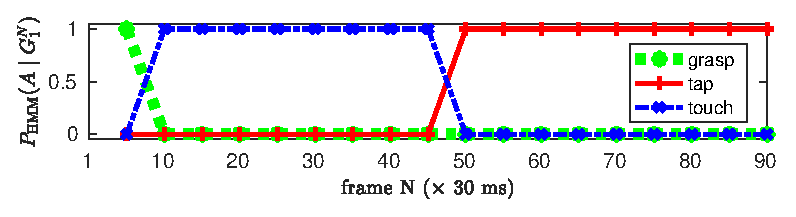
\includegraphics[width=0.7\linewidth]{evolution_of_action_posterior_on_sphere.eps}
    }

    \subfloat[][Prediction of the movement effect on a small sphere.]{
      % here substitute with tap on sphere
      \includegraphics[width=\myWidth\linewidth]{tap-00000109}
      \includegraphics[width=\myWidth\linewidth]{tap-00000110}
      \includegraphics[width=\myWidth\linewidth]{tap-00000112}
      % here add evolution of action posterior
      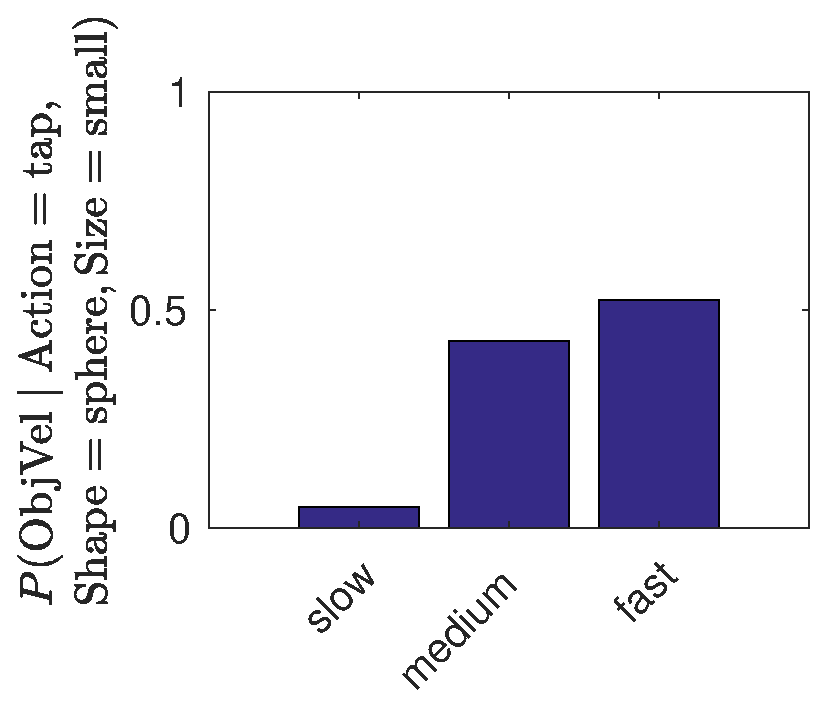
\includegraphics[width=0.20\linewidth]{effectpred_sphere.eps}
      \label{fig:effect_pred:sphere}
    }

    \subfloat[][Prediction of the movement effect on a big box.]{
      \includegraphics[width=\myWidth\linewidth]{tap-00000109}
      \includegraphics[width=\myWidth\linewidth]{tap-00000110}
      \includegraphics[width=\myWidth\linewidth]{tap-00000112}
      % here add evolution of action posterior
      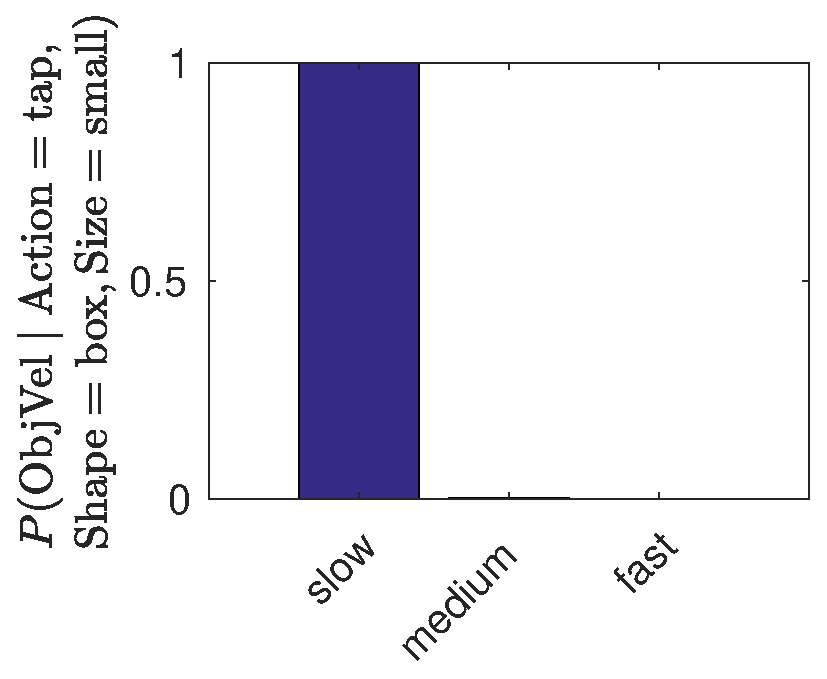
\includegraphics[width=0.20\linewidth]{effectpred_box.eps}
      \label{fig:effect_pred:box}
    }
    \caption{Object velocity predictions, given prior information~(from Gesture \acp{HMM} \emph{hard decision}) that the human user performs a tapping action.}
    \label{fig:effect_pred}
\end{figure*}

NEW RESULT WITH SOFT EVIDENCE (Action)

\begin{figure}
\centering
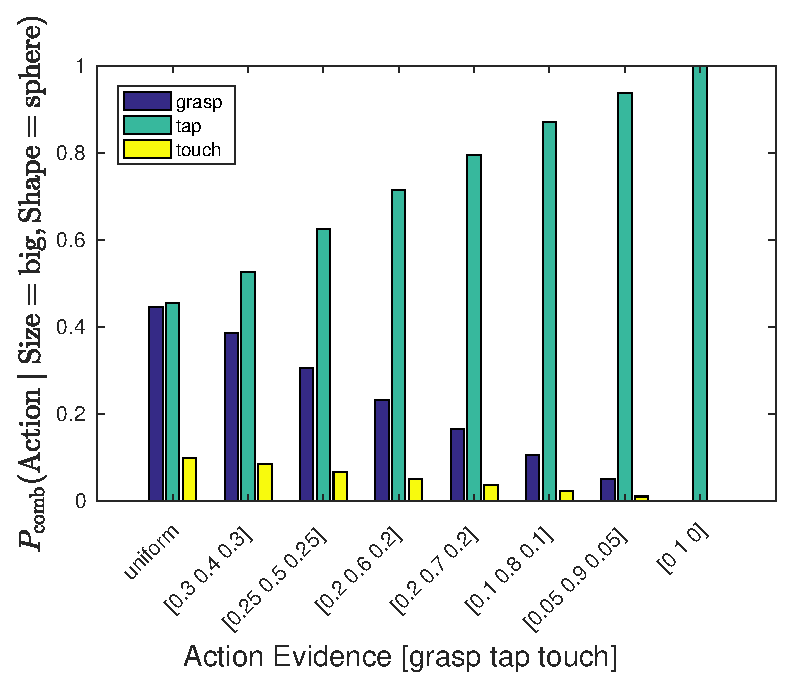
\includegraphics[width=0.9\columnwidth]{impact_of_evidence_on_Action.eps}
\caption{Predictions about the action over a big sphere, when given different probabilistic soft evidence about the action.}
\label{fig:impact_of_evidence_on_Action}
\end{figure}

We now report a result that uses the \emph{soft decision} from the Gesture \acp{HMM}, i.e., the probability distribution over the possible actions.
In Fig.~\ref{fig:impact_of_evidence_on_Action} we show compactly the result of eight different queries~(each group of bars), corresponding to the same number of eight different soft evidences over the action, ranging from a non-informative, uniform distribution~(i.e.,~[1/3~1/3~1/3]), up to the maximum score being attributed to the ``tap'' action~(i.e.,~[0~1~0]), with intermediate distributions in between.
The resulting posterior probability over the Action node is initially ambiguous between ``grasp'' and ``tap'', but then it becomes more and more polarized towards the ``tap'' action as our prior becomes more informative.
This result is not surprising, because the Action node is used both as a prior and as a posterior.
Nonetheless, it serves to validade our formulation for combining different sources of information~(see Sec.~\ref{sec:combination}).

NEW RESULT WITH SOFT EVIDENCE (ObjVel)

\begin{figure*}
\centering
\subfloat[][Predictions about the object velocity of a sphere, when given different probabilistic soft evidence about the action.]
{ 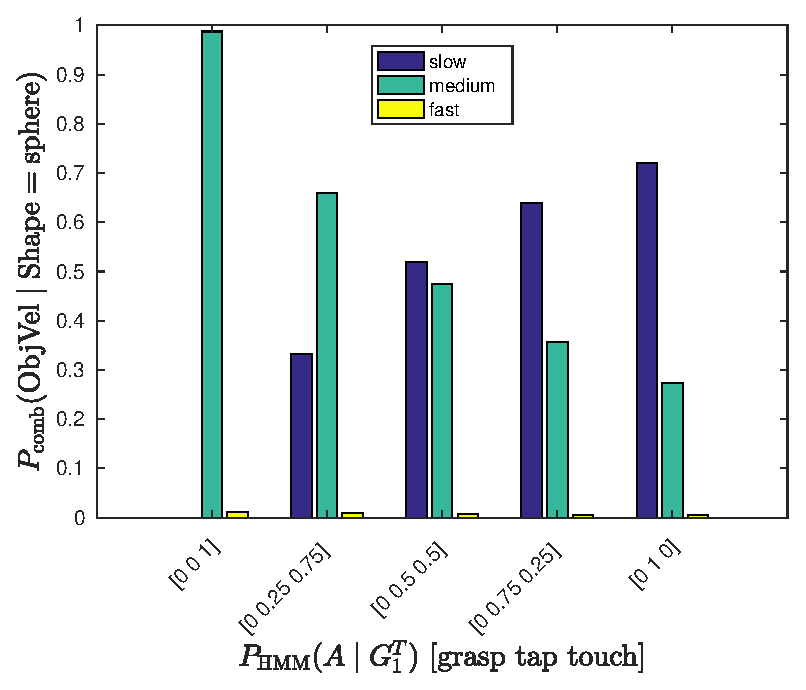
\includegraphics[width=0.45\linewidth]{impact_of_evidence_on_ObjVel_sphere.eps} \label{fig:impact_of_evidence_on_ObjVel_sphere} } \quad
%
\subfloat[][Predictions about the object velocity of a box, when given different probabilistic soft evidence about the action.]
{ 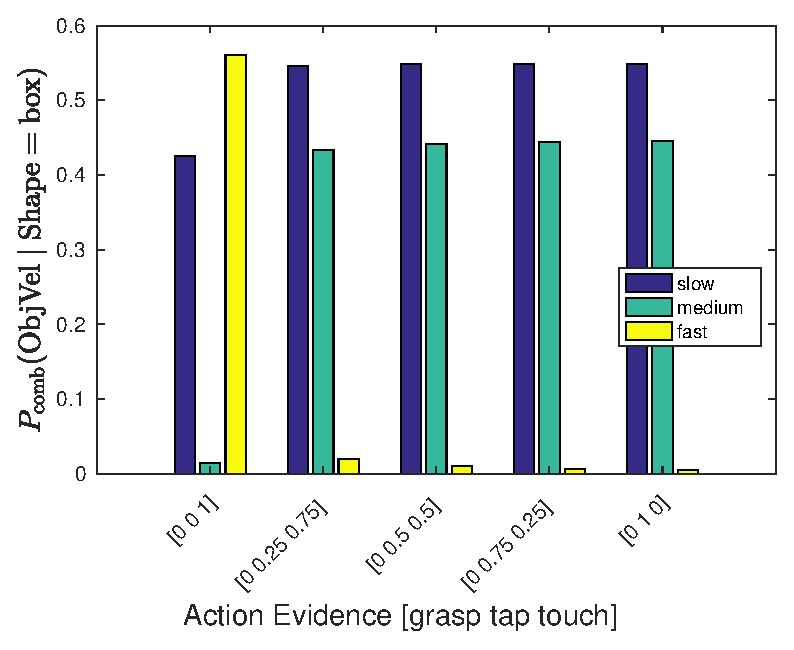
\includegraphics[width=0.45\linewidth]{impact_of_evidence_on_ObjVel_box.eps} \label{fig:impact_of_evidence_on_ObjVel_box} }
\caption{Predictions about the object velocity of different objects, when given probabilistic soft evidence about the action.}
\label{fig:impact_of_evidence_on_ObjVel}
\end{figure*}

Next, we report a result that also uses the \emph{soft decision} over the Action node from the Gesture \acp{HMM}, but this time makes a prediction over a different node: object velocity~(which expresses an effect information).
Fig.~\ref{fig:impact_of_evidence_on_ObjVel} shows the inference in two cases: when the prior information says that the shape is spherical~(see Fig.~\ref{fig:impact_of_evidence_on_ObjVel_sphere}), and when it is cubic~(see Fig.~\ref{fig:impact_of_evidence_on_ObjVel_box}).
TODO complete

\subsection{Prediction of Words}

RESULT FROM GLU WITH HARD EVIDENCE

\begin{figure}
\centering
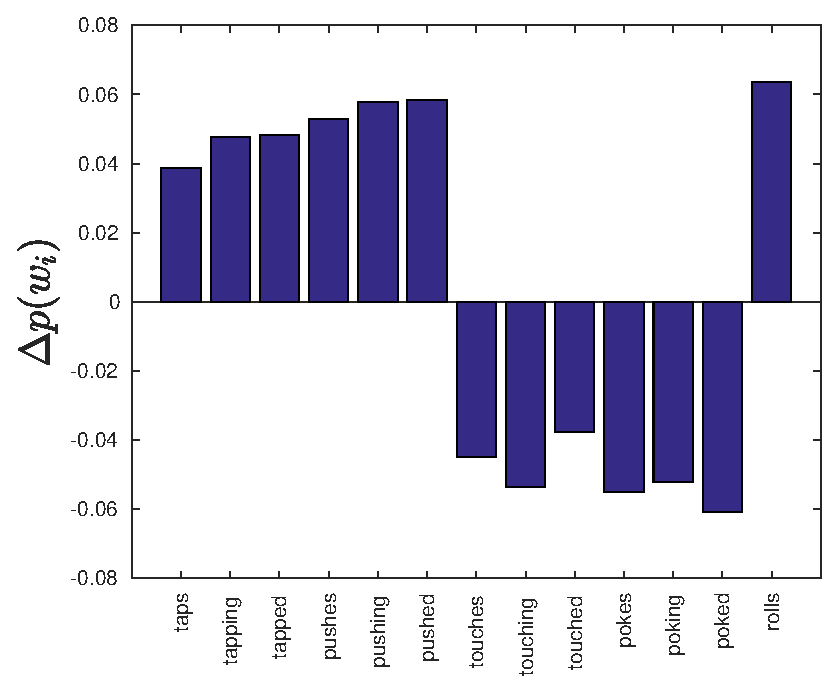
\includegraphics[width=0.9\columnwidth]{partialfig.eps}
\caption{Variation of word occurrence probabilities:
%$\Delta P(w_i) = P(w_i \mid \text{Size=big, Shape=sphere, ObjVel=fast, Action=tap}) - P(w_i \mid \text{Size=big, Shape=sphere,ObjVel=fast})$.
$\Delta P(w_i) = P(w_i \mid \text{InitialEvidence, Action=tap}) - P(w_i \mid \text{InitialEvidence})$, where $\text{InitialEvidence} = \text{Size=big, Shape=sphere, ObjVel=fast}$.
This variation corresponds to the difference of word probability when we add the tap action evidence~(obtained from the Gesture \acp{HMM}) to the initial evidence about object features and effects. We have omitted words for which no significant variation was observed.}
\label{fig:probdiff}
\end{figure}

Our model permits to make predictions over the associated word descriptions in the presence or absence of an action prior.
%As in the previous experiment, we assume that the Gesture \acp{HMM} provide the discrete value of the recognized action performed by a human agent~(i.e., we enforce a hard decision over the observed action).
We compare the associated \emph{verbal description} obtained by the \acl{BN} in the absence of an action prior, with the ones obtained in the presence of one.
In particular, we compare the \emph{probability of word occurrence} resulting from the following two situations:
\begin{enumerate}
%\item when the robot prior knowledge~(evidence in the \ac{BN}) includes information about object features and effects only: \emph{Size=big, Shape=sphere, ObjVel=fast};
%\item when the robot prior knowledge includes, in addition to the above, evidence about the action as observed from the Gestures \acp{HMM}: \emph{Action=tap}.
\item robot prior knowledge evidence consisting of information about object features and effects only: %$\xobs^{\text{before}} = \{ \text{Size=big, Shape=sphere, ObjVel=fast} \}$;
\{Size=big, Shape=sphere, ObjVel=fast\};

\item prior evidence as in the previous situation, with the addition of the action observed from the Gestures \acp{HMM}: %$\xobs^{\text{after}} = \{ \text{Size=big, Shape=sphere, ObjVel=fast, Action=tap} \}$.
\{Size=big, Shape=sphere, ObjVel=fast, Action=tap\}.
\end{enumerate}

Fig.~\ref{fig:probdiff} shows the variation in word occurrence probabilities between the two cases, where we have omitted words for which no significant variation was observed.
We can interpret the difference in the predictions as follows: (i)~as expected, the probabilities of words related to tapping and pushing increase when a tapping action evidence from the Gestures \acp{HMM} is introduced; conversely, the probabilities of other action words~(touching and poking) decreases; (ii)~interestingly, the probability of the word \emph{rolling}~(which is an effect of an action onto an object) also increases when the tapping action evidence is entered. Even though the initial evidence of case~$1$ already included some effect information~(the velocity of the object), it is only now, when the robot perceives that the physical action was a tap, that the event rolling is associated.

\subsection{Verbal Descriptions and Language Properties}

In TODO ADD REF, we have seen how our model is able to generate word probabilities after having received probabilistic observed evidence.
In order to illustrate the capabilities of the model, we use the \ac{CFG} described in Appendix~\ref{appendix:grammar} to generate written descriptions of the robot observations on the basis of the probability distributions of the words inferred by the model.
Note that this grammar is defined here with the only purpose to interpret the probability distributions over the words.
The grammar was neither used in the speech recognition system, nor in learning the associations of the spoken utterances to the affordance variables.
In the model described in~\cite{salvi:2012:smcb}, the speech recognizer used a free loop of words with uniform prior distribution over the words, and the Bayesian model used a bag-of-words assumption, thus disregarding any syntactic information about the spoken descriptions.

During the self-centered learning phase, the verbal descriptions described the agent of the observed actions as either ``the~robot'', ``he'', or ``Baltazar''.
Consequently, the \AffWords{} model learned by the robot includes those words.
In the current study, by merging the \AffWords{} model and the gesture/action recognition model, we allow the robot to reinterpret the concepts it has learned in the self-centered phase, but we do not add any new words to the model.
Consequently, the descriptions that the model generates when observing humans use the same words to describe the agent.

The textual descriptions are generated as follows: given some observed evidence~$\xobs$ that we provide to the model~(hard or soft evidence), we extract the generated word probabilities
%$P(w_i\given \text{evidence})$.
$P(w_i \given \xobs)$.
We generate~$N$ sentences randomly from the \ac{CFG} using the \texttt{HSGen} tool from HTK~\cite{young:htkbook}.
Then, the sentences are re-scored according to the log-likelihood of each word in the sentence, normalized by the length of the sentence:
\begin{equation} \label{eq:sentence_score}
  %\text{score}(s_j\given \text{evidence}) = \frac{1}{n_j} \sum_{k=1}^{n_j} \log P(w_{jk}\given \text{evidence}),
  \text{score}(s_j \given \xobs) = \frac{1}{n_j} \sum_{k=1}^{n_j} \log P(w_{jk} \given \xobs),
\end{equation}
where~$s_j$ is the~$j$th sentence,~$n_j$ is the number of words in the sentence~$s_j$, and~$w_{jk}$ is the~$k$th word in the sentence~$s_j$.
Finally, an $N$-best list of possible descriptions is produced by sorting the scores.

For example, if we provide the following evidence to the model:
\begin{equation} \label{eq:evidence_example}
    \xobs = \{\text{Color=yellow, Size=big, Shape=sphere, ObjVel=fast}\},
\end{equation}
we obtain
%the word probabilities of Fig.~\ref{fig:example_pw} and
the sentences reported in Table~\ref{tab:example_generated_sentences}.
The higher the score, the better.
In the most likely sentence of the list~(in bold), we note that (i)~the correct action-related verb ``taps'' is generated (in the initial evidence, no action information was present, only object features and effects information were), and (ii)~the object term ``ball'' is used twice, both in the first part and in the second part of the sentence (which we can interpret as a coherent choice).

% \begin{figure}
% \centering
% 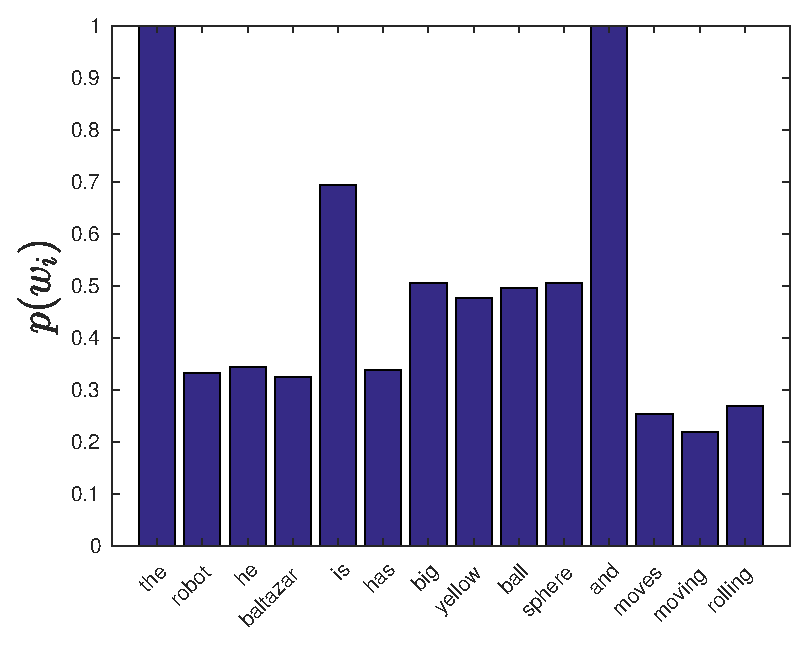
\includegraphics[width=0.9\columnwidth]{example_pw.eps}
% \caption{Word occurrence probabilities given the evidence \emph{\{Color=yellow, Size=big, Shape=sphere, ObjVel=fast\}}. We have omitted words for which no significant probability was observed.}
% \label{fig:example_pw}
% \end{figure}

\begin{table}
    \centering
    \caption{$10$-best list of sentences generated from the evidence~\eqref{eq:evidence_example}.}
    \label{tab:example_generated_sentences}
    \resizebox{\linewidth}{!}{% https://tex.stackexchange.com/a/27105/18819
    \begin{tabular}{ll}
    \toprule
    sentence & score \\
    \midrule
    the robot pushed the ball and the ball moves & $-0.54322$ \\ % not good to have push
    the robot tapped the sphere and the sphere moves & $-0.5605$ \\
    he is pushing the sphere and the sphere moves & $-0.57731$ \\
    the robot is tapping the yellow ball and the big yellow sphere is moving & $-0.57932$ \\
    he pushed the yellow ball and the sphere is rolling & $-0.58853$ \\
    the robot is poking the ball and the sphere is rolling & $-0.58998$ \\
    he is pushing the ball and the yellow ball moves & $-0.59728$ \\
    he pushes the sphere and the ball is moving & $-0.60528$ \\
    he is tapping the yellow ball and the ball is moving & $-0.60675$ \\
    the robot pokes the sphere and the ball is rolling & $-0.60694$ \\
    \bottomrule
    \end{tabular}%
    } % end resizebox
\end{table}

\subsection{Choice of Correct Conjunction}

\newcommand{\evidenceProducingAnd}{Action=grasp, ObjVel=medium}
\newcommand{\evidenceProducingBut}{Action=grasp, ObjVel=slow}

The manipulation experiments that we consider have the following structure: an agent~(human or robot) performs a physical action onto an object with certain properties, and this object will produce a certain physical effect as a result.
For example, ``touch'' on an object yields no physical movement, but ``tap'' does~(especially if the object is spherical).
In the language description associated to an experiment, it makes sense to measure the conjunction chosen by the \acf{CFG} from the observed word probabilities.
In particular, it would be desirable to separate two kinds of behaviors: one in which the action and effect are coherent~(expected conjunction: ``and''), and the other one in which they are contradictory (``but'').

Fig.~\ref{tab:conjunction} shows an example of this behavior of the model.
We give the same action ``grasp'' to the model as evidence, but two values for the final object velocity.
When the object velocity is medium (Fig.~\ref{tab:conjunction:and}), the model interprets this as a successful grasp and uses the conjunction ``and'' to separate the description of the action from the description of the effect.
When the object velocity is slow (in the clustering procedure this was most often zero velocity), the model predicts this is an unsuccessful grasp and uses the conjunction ``but'', instead.

%Example in which the generated conjunction is ``and'' (because of consistency between nodes evidence):
%
%evidence:
%\begin{equation} \label{eq:evidence_producing_and}
%    \xobs^\prime = \{ \text{\evidenceProducingAnd} \}
%\end{equation}

%resulting word probabilities: Fig.~\ref{fig:conjunction_and:pw}

% \begin{figure}
% \centering
% 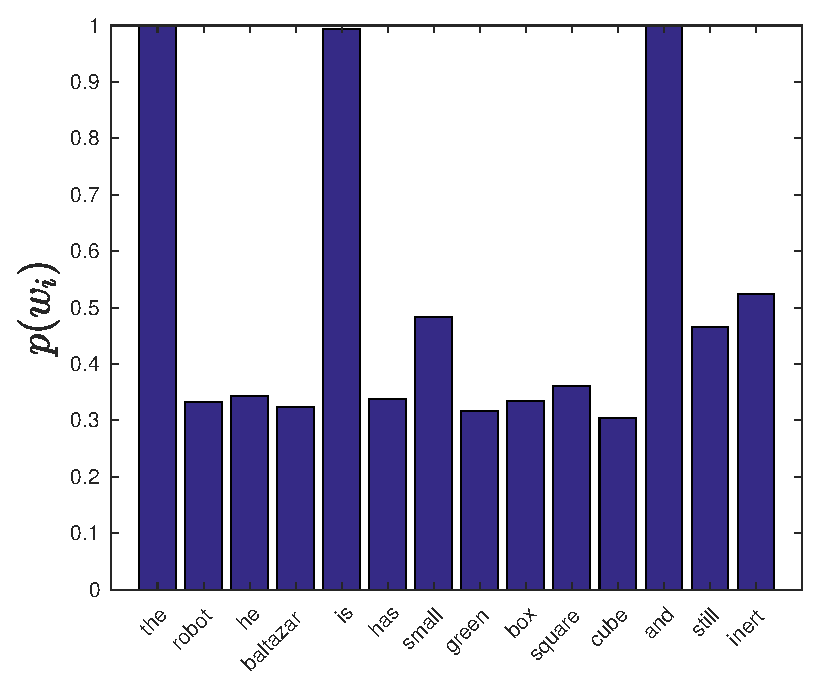
\includegraphics[width=0.9\columnwidth]{and_pw.eps}
% \caption{Word occurrence probabilities given the evidence \emph{\{\evidenceProducingAnd\}}. The ``and'' conjunction has a much higher probability than ``but''. See also Tab.~\ref{tab:conjunction:and}. We have omitted words for which no significant probability was observed.}
% \label{fig:conjunction_and:pw}
% \end{figure}

%generated sentences in Fig.~\ref{tab:conjunction:and}

\begin{figure*}
  \centering
  \subfloat[][Evidence: \evidenceProducingAnd.]{
    \resizebox{!}{0.11\linewidth}{% https://tex.stackexchange.com/a/27105/18819
      \begin{tabular}{ll}
        \toprule
        sentence & score \\
        \midrule
        the robot is picking the sphere \textbf{and} the sphere is moving  & $-0.59328$ \\
        the robot grasps the sphere \textbf{and} the ball is moving  & $-0.59507$ \\
        the robot is picking the sphere \textbf{and} the sphere is rising  & $-0.60882$ \\
        the robot grasped the sphere \textbf{and} the sphere is rising  & $-0.61842$ \\
        the robot picked the ball \textbf{and} the ball is rising  & $-0.64052$ \\
        baltazar grasps the sphere \textbf{and} the sphere is moving  & $-0.66182$ \\
        the robot has grasped the ball \textbf{and} the ball is rising  & $-0.66398$ \\
        the robot picked the ball \textbf{and} the green ball is moving  & $-0.67134$ \\
        baltazar grasped the sphere \textbf{and} the ball is moving  & $-0.67283$ \\
        baltazar is grasping the ball \textbf{and} the sphere is rising  & $-0.6787$ \\
        \bottomrule
      \end{tabular}%
    } % end resizebox
    \label{tab:conjunction:and}
  } % end subfloat
  \subfloat[][Evidence: \evidenceProducingBut.]{
    \resizebox{!}{0.11\linewidth}{% https://tex.stackexchange.com/a/27105/18819
      \begin{tabular}{ll}
        \toprule
        sentence & score \\
        \midrule
        the robot is picking the cube \textbf{but} the square is still  & $-0.52575$ \\
        the robot is grasping the sphere \textbf{but} the box is inert  & $-0.55$ \\
        the robot is grasping the square \textbf{but} the sphere is still  & $-0.55388$ \\
        the robot grasped the square \textbf{but} the cube is inert  & $-0.55608$ \\
        baltazar is grasping the square \textbf{but} the square is inert  & $-0.5571$ \\
        the robot is grasping the cube \textbf{but} the ball is inert  & $-0.56011$ \\
        the robot picks the box \textbf{but} the square is inert  & $-0.56397$ \\
        baltazar is picking the square \textbf{but} the square is still  & $-0.56402$ \\
        he is grasping the square \textbf{but} the cube is inert  & $-0.56815$ \\
        the robot grasps the square \textbf{but} the sphere is inert  & $-0.57417$ \\
        \bottomrule
      \end{tabular}%
    } % end resizebox
    \label{tab:conjunction:but}
  } % end subfloat
%    \caption{Top sentences generated from the evidence~~\eqref{eq:evidence_producing_and}. The ``and'' conjunction was chosen in all of them. Intuitively, the model has learned that a grasping action which produces a significant movement is successful.}
%    \label{tab:conjunction:and}
%
%    \centering
    \caption{$10$-best list of sentences generated given two different sets of evidence.
    In~(a) the model interprets the object movement as indicating a succesful grasp and uses the conjunction ``and''.
    In~(b) the slow movement is interpreted as no movement at all, and, therefore, as an unsuccessful grasp: as a result, the conjunction ``but'' is used.}
    \label{tab:conjunction}
\end{figure*}


%Example in which the generated conjunction is ``but'' (because of no consistency):
%
%evidence:
%\begin{equation} \label{eq:evidence_producing_but}
%    \xobs'' = \{ \text{\evidenceProducingBut} \}
%\end{equation}

%resulting word probabilities: Fig.~\ref{fig:conjunction_but:pw}

% \begin{figure}
% \centering
% \includegraphics[width=0.9\columnwidth]{but_pw.eps}
% \caption{Word occurrence probabilities given the evidence \emph{\{\evidenceProducingBut\}}. The conjunctions ``and'' and ``but'' have comparable probabilities, with the former being slightly higher. See also Tab.~\ref{tab:conjunction:but}. We have omitted words for which no significant probability was observed.}
% \label{fig:conjunction_but:pw}
% \end{figure}

%generated sentences in Fig.~\ref{tab:conjunction:but}

% A clarification is due: even though the conjunction ``and'' is still the most likely, the conjunction ``but'' has a comparable probability, given the observed evidence~(see Fig.~\ref{fig:conjunction_but:pw}).
% Even so, ``but'' was chosen in the highest-ranked sentence and in two more of the top-ten sentences~(see Tab.~\ref{tab:conjunction:but}).
% This result can be loosely interpreted as TODO

\begin{figure}
\centering
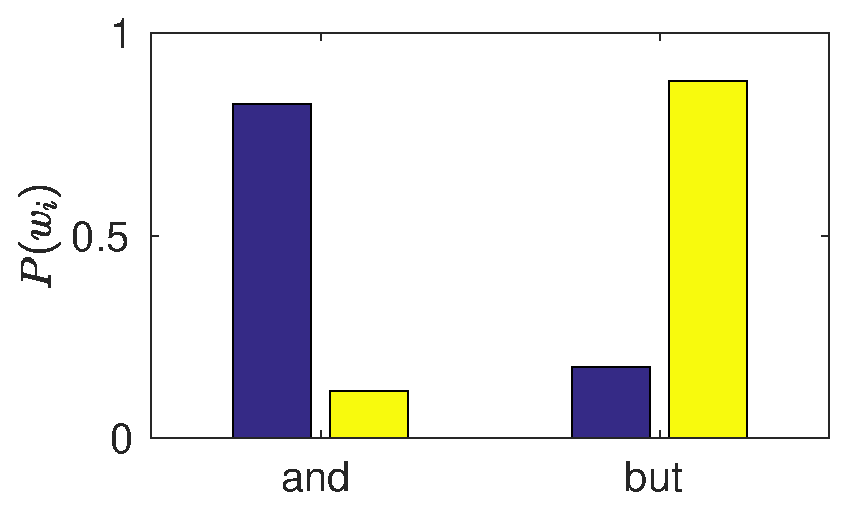
\includegraphics[width=0.9\columnwidth]{p_conjunctions.eps}
\caption{Word occurrence probabilities of the conjunctions ``and'' and ``but'' obtained when entering a consistent \actioneffect{} evidence vs when entering an inconsistent \actioneffect{} evidence. See Fig.~\ref{tab:conjunction} for details.}
\label{fig:p_conjunctions}
\end{figure}

\subsection{Solving Ambiguities with the Combined Model}

Fig.~\ref{fig:update_from_softevidence} shows the result of predictions over nodes given some (hard) evidence, before and after incorporating further soft evidence

\begin{figure*}
    \centering
    \subfloat[][Prediction of the model given the initial (hard) evidence. The prediction is ambiguous.]
    { 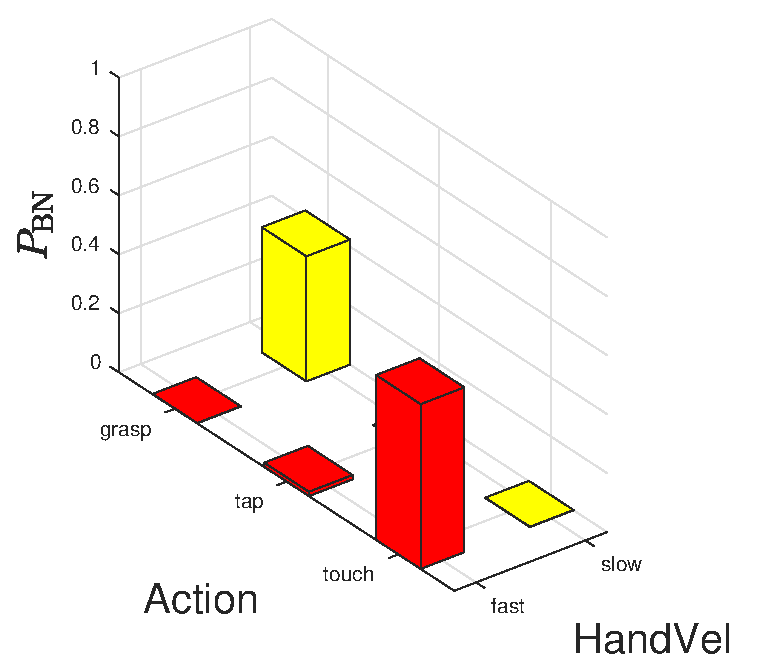
\includegraphics[width=0.45\linewidth]{before_softevidence_prediction.eps} \label{fig:before_softevidence:pred} } \quad
    %
    \subfloat[][Updated prediction of the model after having incorporated the Action soft evidence (grasp tap touch)=(0.8 0.1 0.1) TODO IMPROVE NOTATION. The prediction is now unambiguous.]
    { 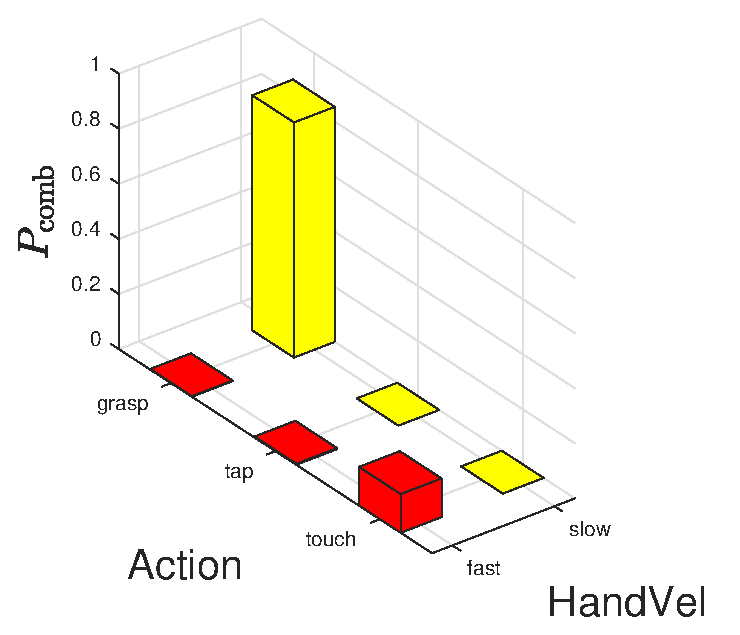
\includegraphics[width=0.45\linewidth]{after_softevidence_prediction.eps} \label{fig:after_softevidence:pred} }
    \caption{Predictions about the action and hand velocity on a box object, before and after incorporating Action soft evidence from Gesture \acp{HMM}.}
    \label{fig:update_from_softevidence}
\end{figure*}

word probabilities: Fig.~\ref{fig:after_softevidence:pw} (in this case they are identical before and after incorporating the soft evidence)

\begin{figure}
\centering
\includegraphics[width=0.9\columnwidth]{after_softevidence_pw.eps}
\caption{Word occurrence probabilities given the evidence \{Shape=box, ObjVel=fast\}. We have omitted words for which no significant probability was observed.}
\label{fig:after_softevidence:pw}
\end{figure}


%%%%%%%%%%%%%%%%%%%%%%%%%%%%%%%%%%%%%%%%%%%%%%%%%%%%%%%%%%%%%%%%%%%%%%%%%%%%%%%%
%!TEX encoding = UTF-8 Unicode

\section{Conclusions and Future Work}

Future work:
\begin{itemize}
  \item possibility to add new vocabulary words to the system
\end{itemize}

Things we need to discuss:
\begin{itemize}
\item the effect variables in the BN include hand velocity. How does this relate to the gesture features in the HMM? Can we learn the connection?
\item in order to achieve the ideal case in Figure~\ref{fig:model} we would need to learn the complex relationship between hand movements and affordance variables:
  \begin{itemize}
  \item how can this be achieved in the ego-centric learning? Mixture of HMMs and BN? Would it be possible to learn the dependency structure in this complex model?
  \item assuming it is possible to learn in the ego-centric way, how can this be extended to the other agent? Coordinates will definitely be different. In the current study we could directly map the two because we were using the categorical variable ``action''.
  \end{itemize}
\end{itemize}

BELOW IS THE GLU TEXT

Within the scope of cognitive robots that operate in unstructured environments, we have discussed a model that combines word affordance learning with body gesture recognition. We have proposed such an approach, based on the intuition that a robot can generalize its previously-acquired knowledge of the world~(objects, actions, effects, verbal descriptions) to the cases when it observes a human agent performing familiar actions in a shared \hr{} environment. We have shown promising preliminary results that indicate that a robot's ability to predict the future can benefit from incorporate the knowledge of a partner's action, facilitating scene interpretation and, as a result, teamwork.

In terms of future work, there are several avenues to explore. The main ones are (i)~the implementation of a fully probabilistic fusion between the affordance and the gesture components~(e.g., the soft decision discussed in Sec.~\ref{sec:combination}); (ii)~to run quantitative tests on larger corpora of \hr{} data; (iii)~to explicitly address the correspondence problem of actions between two agents operating on the same world objects~(e.g., a pulling action from the perspective of the human corresponds to a pushing action from the perspective of the robot, generating specular effects).


%%%%%%%%%%%%%%%%%%%%%%%%%%%%%%%%%%%%%%%%%%%%%%%%%%%%%%%%%%%%%%%%%%%%%%%%%%%%%%%%
\section*{Acknowledgments}

This work was partially supported by the FCT project~UID/EEA/50009/2013 and by the CHIST-ERA project IGLU.

%%%%%%%%%%%%%%%%%%%%%%%%%%%%%%%%%%%%%%%%%%%%%%%%%%%%%%%%%%%%%%%%%%%%%%%%%%%%%%%%
\printbibliography

\appendix
%%%%%%%%%%%%%%%%%%%%%%%%%%%%%%%%%%%%%%%%%%%%%%%%%%%%%%%%%%%%%%%%%%%%%%%%%%%%%%%%
\section{Grammar Definition}
\label{appendix:grammar}
Below, we provide the grammar definition used to generate verbal descriptions from the probability distribution over words estimated by the model.
Note, however, that no grammar was used during the learning phase: the speech recognizer used as a frontend to the spoken descriptions is based on a loop of words with no grammar, and the \AffWords{} model is based on a bag-of-words assumption, where only the presence or absence of each word in the description is considered.

\begin{figure}
  \includegraphics[width=\textwidth, angle=90]{figures/grammar}
  \caption{Graphical representation of the formal \acf{CFG} used to generate descriptions from word probability distribution.}
  \label{fig:grammar}
\end{figure}

\begin{grammar}
  <agent> ::= the robot | he | baltazar

  <size> ::= big | small

  <color> ::= green | yellow | blue

  <shape> ::= sphere | ball | cube | box | square

  <object> ::= the [<size>] [<color>] <shape>

  <touch> ::= touches | [has] [just] touched | is touching

  <poke> ::= pokes | [has] [just] poked | is poking

  <tap> ::= taps | [has] [just] tapped | is tapping

  <push> ::= pushes | [has] [just] pushed | is pushing

  <grasp> ::= grasps | [has] [just] grasped | is grasping

  <pick> ::= picks | [has] [just] picked | is picking

  <action> ::= <touch> | <poke> | <tap> | <push> | <grasp> | <pick>

  <conjunction> ::= and | but

  <inertmove> ::= is inert | is still | moves | is moving

  <slideroll> ::= slides | is sliding | rolls | is rolling

  <fallrise> ::= rises | is rising | falls | is falling

  <effect> ::= <inertmove> | <slideroll> | <fallrise>

  <sentence> ::= <agent> <action> <object> <conjunction> <object> <effect>
\end{grammar}

Given a probability distribution over the words,~$P(w_i)$, a number~$N$ of sentences is randomly generated from the grammar using the \texttt{HSGen} tool from HTK~\cite{young:htkbook}.
Then, the sentences are re-scored according to the log-likelihood of each word in the sentence, normalized by the length of the sentence.
Finally, an $N$-best list of possible descriptions is produced by sorting the scores.

\begin{equation*}
  \text{score}(s_j) = \frac{1}{n_j} \sum_{k=1}^{n_j} \log P(w_{jk}),
\end{equation*}
where~$s_j$ is the~$j$th sentence,~$n_j$ is the number of words in the sentence~$s_j$, and~$w_{jk}$ is the~$k$th word in the sentence~$s_j$.


\end{document}
